% Impedanz-Ortskurve und Admittanz-Ortskurve von RLs-Glied (omega als Parameter)
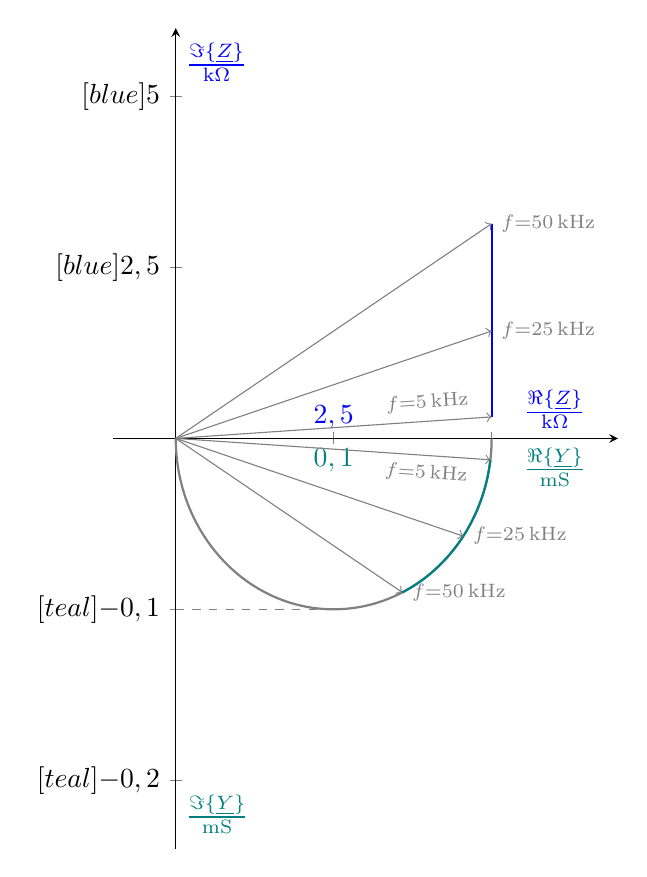
\begin{tikzpicture}
    \begin{axis}[
        axis lines=center,
        xmin=-1,xmax=+7,% x=1 = 1 kOhm = 0,1 mS
        ymin=-6,ymax=+6,% y=1 = 1 kOhm = 0,1 mS
        xtick={-5,-2.5,2.5,5},
        ytick={-5,-2.5,2.5,5},
        xticklabels={},
        yticklabels={$\ec[teal]{-0,2}$,$\ec[teal]{-0,1}$,$\ec[blue]{2,5}$,$\ec[blue]{5}$},
        width=8cm, height=12cm,%
    ]
        % axis-labels
        \draw (0,+5.5) node[blue, right]{$\frac{\Im\{\underline{Z}\}}{\mathrm{k}\Omega}$};
        \draw (6, 0.0) node[blue, above]{$\frac{\Re\{\underline{Z}\}}{\mathrm{k}\Omega}$};
        \draw (0,-5.5) node[teal, right]{$\frac{\Im\{\underline{Y}\}}{\mathrm{mS}}$};
        \draw (6, 0.0) node[teal, below]{$\frac{\Re\{\underline{Y}\}}{\mathrm{mS}}$};
        % x-axis ticks
        \draw (2.5,0) node[blue, above]{$2,5$};
        \draw (2.5,0) node[teal, below]{$0,1$};
        % Ortskurven
        \addplot[mark=none,thick,blue] coordinates{(5,+0.31416)(5,+3.1416)}; % Z
        \draw[mark=none,thick,gray] (+5.00,-0.00000) arc[start angle=-0.000, end angle=-180.0, radius=2.5];
        \draw[mark=none,thick,teal] (+4.98,-0.31416) arc[start angle=-7.162, end angle=-64.28, radius=2.5]; % julia: angle(1000/(5000+2pi*5000*0.01*im)*25-2.5)*360/(2pi)
        \addplot[dashed, gray] coordinates{(0,-2.5)(2.5,-2.5)}; % Hilfslinie um Radius abzulesen
        % Zeiger
        \addplot[->,gray] coordinates{(0,0)(5,+0.31416)} node[pos=0.8, left, above, sloped]{$\scriptstyle{f= 5\,\mathrm{kHz}}$};
        \addplot[->,gray] coordinates{(0,0)(5,+1.5708)}  node[pos=1.0, left, right]{$\scriptstyle{f=25\,\mathrm{kHz}}$};
        \addplot[->,gray] coordinates{(0,0)(5,+3.1416)}  node[pos=1.0, left, right]{$\scriptstyle{f=50\,\mathrm{kHz}}$};
        \addplot[->,gray] coordinates{(0,0)(4.980,-0.313)} node[pos=0.8, left, below, sloped]{$\scriptstyle{f= 5\,\mathrm{kHz}}$};
        \addplot[->,gray] coordinates{(0,0)(4.551,-1.430)}  node[pos=1.0, left, right]{$\scriptstyle{f=25\,\mathrm{kHz}}$}; 
        \addplot[->,gray] coordinates{(0,0)(3.585,-2.252)}  node[pos=1.0, left, right]{$\scriptstyle{f=50\,\mathrm{kHz}}$};
\end{axis}
\end{tikzpicture}
